% Chapter 1

\chapter{Introduction} % Write in your own chapter title
\label{Chapter1}
% \lhead{Chapter 1. \emph{Introduction}} % Write in your own chapter title to
\fancyhead[RO,LE]{Chapter 1. Introduction} % for double sided printing
\fancyhead[RE,LO]{\thepage}
% Task: port stuff to other chaps; make this ultra-short.
The research presented in this thesis focuses on commuting and its energy costs.
UK datasets from the beginning of the 21$^{st}$ century form the empirical
foundation of the work. Travel to work statistics are described, analysed and in later
chapters modelled to assess the variability of energy use for this commuting.
The underlying motivations are broader and play an important role
throughout the thesis, from the choice of methodology (\cref{Chapter4}) to the
specification for scenarios of change (\cref{Chapter8}).
% The premise of the research, that energy use is an important measure of
 % travel systems, is based on evidence from a range of disciplines.
% including
% climate science, `peak oil' theory and social sciences.
% The thesis is framed in terms of these big issues
% The thesis is policy-driven.
It is therefore important to lay out these wider issues at the outset, before
highlighting the impact of commuting at the individual and national scale (in
sections \ref{s:realities} and \ref{snimportance}). These `big picture'
motivations also inform the research aims and objectives (\cref{s:aims}).

\section{The `Big Picture'}
% In the grand scheme of things the topic of this work ---
%  commuting and its energy impacts --- may seem mundane.
% The issues that it relates to are big, however.
Our increasingly interconnected global civilisation is facing challenges
that are unique in the history of humankind. Environmental
and social-economic changes are occurring to a greater extent and faster
than ever before \citep{Rifkin2011a, ehrlich2013can}. Perhaps more
importantly, this generation is in the privileged position of being able to monitor,
predict and respond to these changes as they occur \citep{Evans1998,
Smil2008, IPCC2007}.
This work is firmly situated in the context of these changes and aims to
contribute to humanity's understanding of them.
Following the academic tendency for specialisation
 whilst avoiding the pitfalls of dogmatic allegiance to any particular
discipline or worldview \citep{kates1986geography},
this thesis focuses on one `bite-sized' yet important part of these wider
issues.

Energy intensive transport
contributes to pressing environmental, social and economic problems of the
21$^{st}$ century. Climate change, resource depletion, and growing levels of
economic inequality are global problems aggravated by energy use.
Travel is a major energy consumer. Yet transport
systems powered by fossil fuels have become integral to modern life:
by the 1970s `automobility' was central to social change \citep{Illich1974}
and since then motorised transport has become even more central to
modern life \citep{Rodrigue2009}.
This means that policy-makers, businesses, and individuals
 will have to make difficult decisions in the coming decades.
According to some the situation is urgent: ``Rapid decisions now need to
be made
so that the impacts of transport on the environment can be minimised and fossil
fuel resources conserved'' \citep[p.~354]{Chapman2007}. \emph{Rapid} decisions are not
always \emph{good} decisions, however: rational choices depend on good
information about the world.
 %Expand and quote from Illich

Because of the scale and complexity of the previously mentioned global
problems, it is temping to focus solely on the detail of energy use in commuting
 as one aspect of personal travel about which good datasets are available.
% it is
%tempting to focus on the detail --- in this case
%the abstract and reductionist energy costs of one source of personal travel:
%transport to work. 
It is however important to understand the wider context of 
transport energy use in order to decide the most useful applications of and
directions for future research in this area.
%However, an understanding of the context in which interest
%in transport energy use has grown is vital to deciding which research
%directions to pursue. Understanding of this wider context also informs
%how the methods and understanding contained in this
%narrow field of knowledge can best be mobilised.
%  to
% inform people who must make decisions now that will based on an uncertain future.
An introduction to the broader context that motivates this research is therefore
provided, focussing on the three `big issues' of climate change, peak oil,
and economic inequality which are also
long-term political priorities in the UK \citep{UKERC2010}.

\subsection{Climate change}
The Earth's climate has always changed: it is a complex system with non-linear
responses to internal and external drivers and a number of feedback loops
\citep{IPCC2007}. The changes during the 20$^{th}$ and 21$^{st}$ centuries are,
however, different from those observed in the paleoclimate record: ``It is
important to realize that the
current change in atmospheric CO$_{2}$ is proceeding at a rate more than 200
times faster than any natural change in Earth's past history with the exception
of the Cretaceous-Tertiary boundary event generally attributed to impact of an
asteroid with the Earth'' \citep{Hay2011}. The other major difference is that
today climate change is caused by the combustion of fossil fuels by humans.
Commuting, composed of millions of motorised trips to work and back each day, is
a small yet important contributor. The desire to reduce these emissions, for the
maintenance of a ``safe operating space for humanity'' \citep{Rockstrom2009}
provides an important motivation for this research. An underlying aim is to
contribute ideas and information to the ongoing debate about how to mitigate
anthropogenic climate change \citep{Matschoss2011}.


This aim appears to be shared by others:
academic interest in transport emissions has proliferated in recent years
\citep{Akerman2006, Chapman2007, Schwanen2011}, although less so in the
specific area of commuting (\cref{Chapter2}).
Because energy use is directly related to greenhouse gas
emissions \citep{MacKay2009}, this research is also about climate change.
%%% The following is superfluous bollocks!
% Before presenting the other major policy driver of this research, energy
% security, it is important to understand how emissions relate to the UK's
% climate change policy. This is the subject of the next subsection. 

\subsubsection*{UK greenhouse gas emissions}
At the UK level, the emissions associated with commuter energy are subsumed
within `transport emissions'. These include emissions from shipping, aviation
and military transport, as well as the road and rail sectors
\citep{Decc2011t}. Road transport dominates,
accounting for more than 90\% of the UK's transport emissions
(\cref{fig:cc-trans}).

\begin{figure}[h]
 \centering
 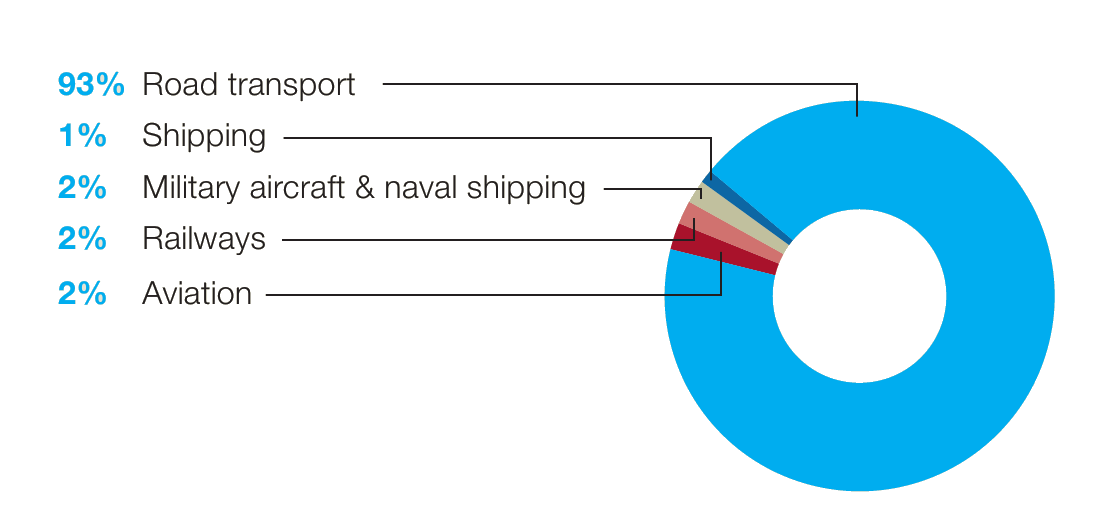
\includegraphics[width=14cm]{cc-trans.png}
 % cc-trans.png: 1113x529 pixel, 72dpi, 39.26x18.66 cm, bb=0 0 1113 529
 \caption{UK transport emissions by source in 2009 \citep{Decc2011t}.}
 \label{fig:cc-trans}
\end{figure}

An interesting feature of the UK's emissions reporting strategy is that
`transport' is generally presented as a monolithic category (e.g.
\citealp{Decc2010}), despite the wide variety of transport modes and purposes
presented in \cref{fig:cc-trans}. This makes it difficult to identify the
specific drivers of growth in UK transport emissions since 1970
\citep{Gasparatos2009} and stagnation since 1990 (\cref{fig:cc-ems}).
What is clear in
both cases is that energy use and hence emissions from transport have increased
(since 1970) or stagnated (since 1990) while those of other sectors have
declined. Between 1990 and 2010, transport was the only sector other than
housing in which emissions increased; transport now accounts for just over 20\%
of UK emissions (\cref{table:mtco2}, below). This research project quantifies
the contribution of commuting to this total in terms of energy use, and provides evidence
about which strategies may be effective for reducing the emissions due to
transport to work.

The UK's climate change commitments are unambiguous, agreed upon by all major
parties, and legally binding: emissions in 2050 must be below 20\% of their 1990
level \citep{ClimateChangeAct2008}. This means that the \emph{total}
permitted emissions in 2050 across all sectors are roughly equal to the emissions from
just the \emph{transport sector} today. This fact underlines the scale of the
proposed changes: transport to work represents a small but important component
of this challenge that affects millions of working people every day.

\begin{figure}[h]
 \centerline{
 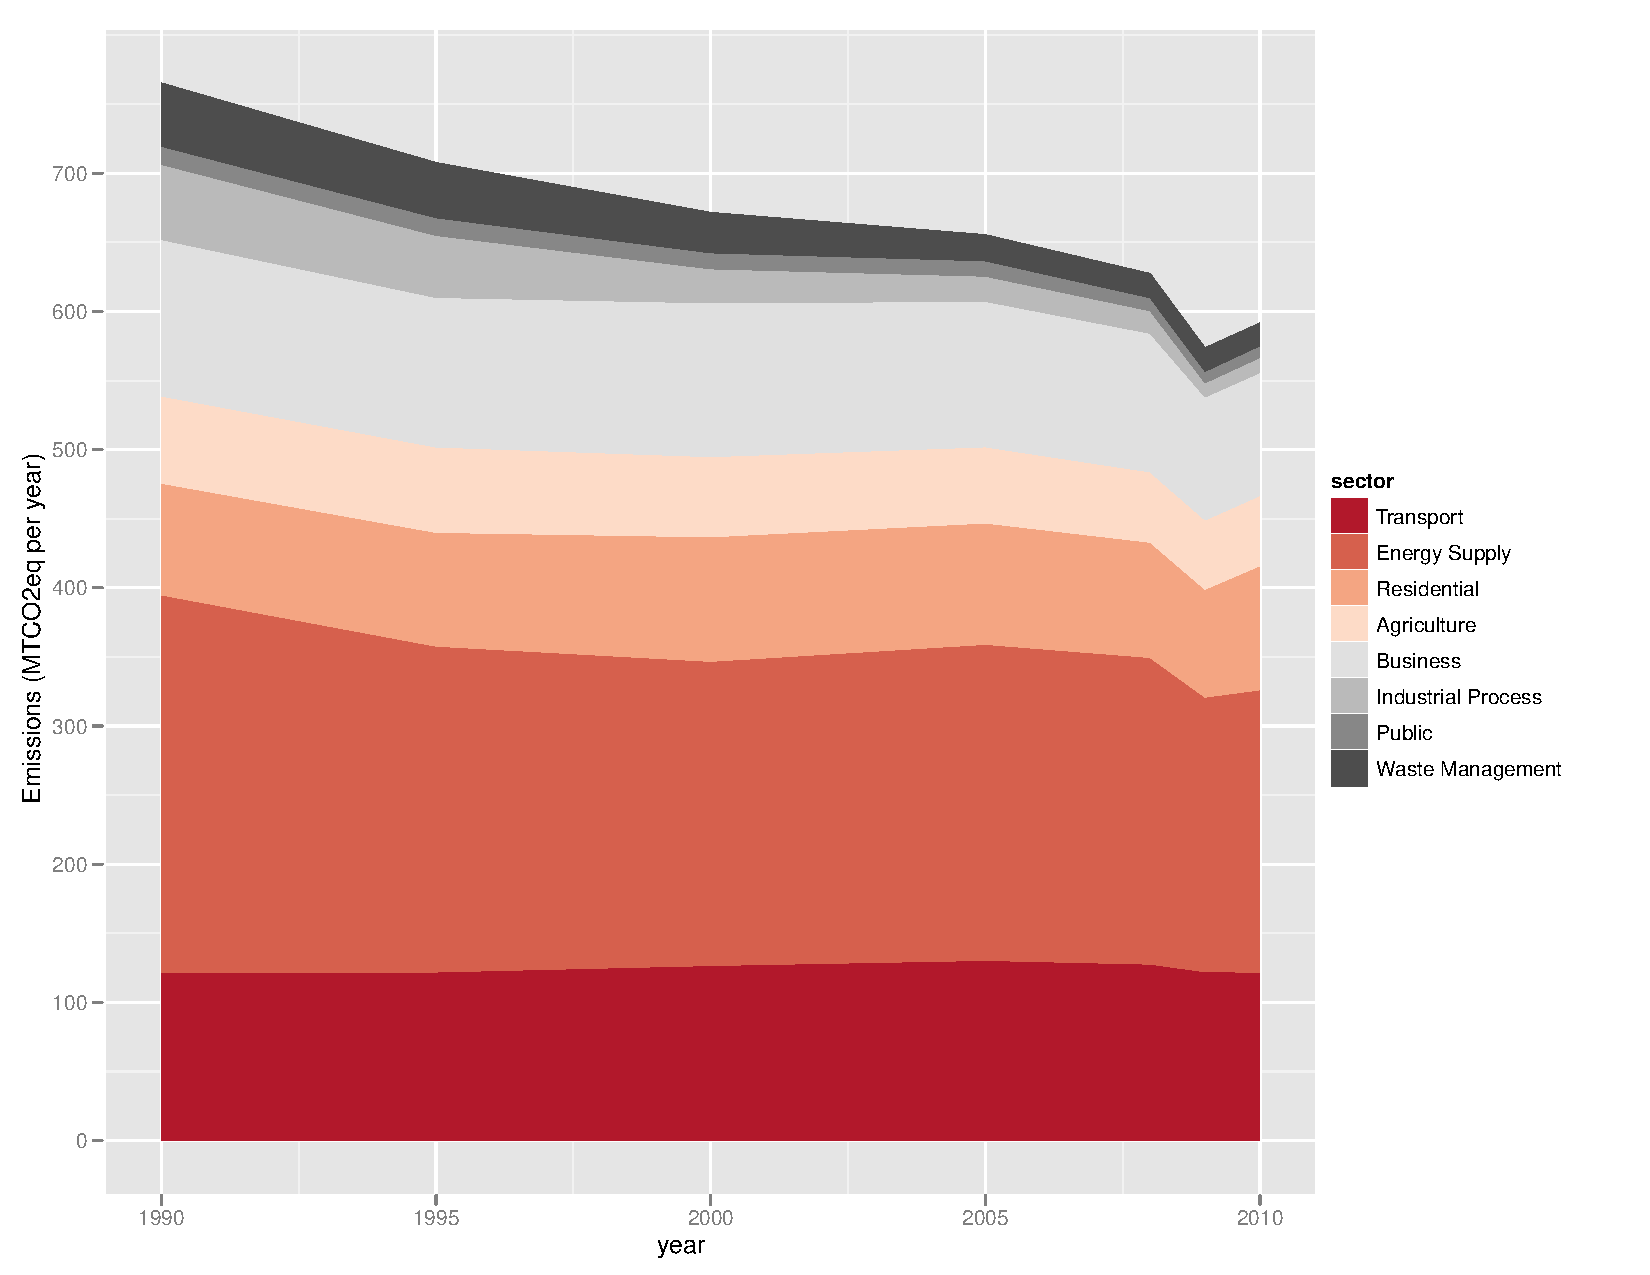
\includegraphics[width=17 cm,bb=0 0 792 612]{cc-ems.pdf}}
 % cc-ems.pdf: 792x612 pixel, 72dpi, 27.94x21.59 cm, bb=0 0 792 612
\caption{UK greenhouse gas emissions by sector. Data from
 \citet{Decc2011ff}.}
 \label{fig:cc-ems}
\end{figure}

\begin{table}[htbp]
\caption[Top 5 UK sectors in terms of greenhouse gas emissions, 1990-2010]{Top 5
UK sectors in terms of greenhouse gas emissions, 1990-2010
(MtCO$_{2}$e). Data from \citet{Decc2011ff}}
\centering{
\begin{tabular}{lrrrrr}

 & 1990 & 2000 & 2010 & \multicolumn{1}{l}{\% change} & \multicolumn{1}{l}{\%
emissions (2010)} \\ \hline
Energy Supply & 273.4 & 220.1 & 204.3 & -25.3 & 34.8 \\ \hline
Transport & 121.5 & 126.7 & 121.9 & 0.3 & 20.7 \\ \hline
Residential & 80.8 & 90.1 & 89.9 & 11.3 & 15.3 \\ \hline
Business & 113.2 & 111.3 & 89 & -21.4 & 15.1 \\ \hline
Agriculture & 63.1 & 58 & 50.7 & -19.7 & 8.6 \\ \hline
Other & 117.4 & 65.8 & 32 & -72.7 & 5.4 \\ \hline
Total & 769.4 & 672 & 587.8 & -23.6 & 100.0 \\ \hline
\end{tabular}
}
\label{table:mtco2}
\end{table}

\subsubsection*{Emissions from transport to work}
% Something about transport being a challenging sector for emissions cuts
% Something about freight vs personal transport energy use and emissions
Of the 20\% of UK emissions that arise from transport, only a small fraction
are due to transport to work. How small? No official breakdowns of emissions are
provided by reason for trip, but estimates can be made by
analysing the make-up of the transport sector. As shown in 
\cref{fig:cc-trans}, 5\% of transport emissions can be accounted for by military
vehicles, aviation and shipping: none of these are usually involved in transport to
work. Also, 31\% of road transport emissions arise from goods vehicles (HGVs and
LGVs); the remaining 69\% arise from road vehicles for personal transport --
buses, motorcycles and cars \citep{DECC2011a}. From these figures, it is
possible to estimate that ~80 MtCO$_{2}$e result from personal travel in the UK.
19.5\% of passenger kilometres travelled by all personal transport modes in the
UK are due to travel to work \citep{DfT2011-why}. Transport to work
can be estimated to cause $\sim$16 MtCO$_{2}$e of emissions or around 3\% of the
UK's total. (In \cref{stotalcomp} a more refined estimate of commuter energy
use is presented, based
on geographically disaggregated data: commuting was found to account for
4.1\% of total energy use and 14.4\% of transport energy use.)

It is important to undertake such `back of the
envelope' calculations at the outset of research into emissions reduction
strategies or sustainable energy to ensure that time is not wasted on negligible
issues such as phone chargers \citep{MacKay2009}. David MacKay, Chief Scientific
Advisor at the Department of Energy and Climate Change (DECC), puts this
argument in lay terms by proposing a rule for
energy-saving interventions: ``A gizmo may be discussed only if it could lead to
energy savings of at least 1\% ... because the public conversation about energy
surely deserves to be
focussed on bigger fish'' \citep{MacKay2009-energyplates}. Applying this
reasoning more broadly to areas of energy use, transport to work clearly
deserves attention according to
this rule, although emissions cuts in commuting will have to be matched in all
other sectors for targets to be met. However, there are reasons to believe that
making cuts in the transport sector generally, and in transport to work in
particular, will be especially difficult, and therefore worthy of dedicated
investigation. These include:
\begin{itemize}
\item The transport sector is overwhelmingly dependent on petrol and diesel:
motorised transport (which accounts for most trips and the vast majority of the
distance travelled, as shown in \cref{Chapter5}) is 95\% %really!!!
dependent on refined oil products \citep{Woodcock2007}. This is problematic
because there are no commercially viable, low emissions alternatives to crude
oil for liquid fuels. Biofuels are the only `renewable' option on the table,
but their potential contribution is low \citep{Patzek2006,Michel2012}, they
can conflict with
food production \citep{Pimentel2009}, and currently used crops may increase
greenhouse gas emissions due to land use change \citep{Fargione2008}.
\item Linked with the previous point, low carbon technology is far less
promising in the transport sector than in other large emitting sectors.
% In electricity generation and residential heat demand, for example the %dad'd
For electricity generation and residential heating the technologies
for renewable alternatives are becoming more commercially viable \citep{Chu2012}.
By contrast,
the penetration of electric, hydrogen, and biofuel-powered cars may be slow,
largely due to their high cost \citep{Proost2011,AdamVaughan2011}.
\item The current transport system is built around road (and to a lesser extent
rail) infrastructure that took many decades and large capital investments to
complete. The dependence of society on the car is deeply embedded, yet a
low-energy (and hence low emissions) transport system may require a shift away
from personal ownership of automobiles altogether
\citep{MacKay2009,Moriarty2010}, something that will take decades to accomplish.
\end{itemize}
These difficulties make de-carbonising transport systems problematic
compared with the other large energy users --- electricity and heat
production.\footnote{These can convert more easily to renewable
sources --- e.g.~via stationary wind turbines
and solar hot water panels --- than can transport systems.
This is because transport systems are inherently mobile,
therefore requiring high energy density energy storage.
Fossil fuels are unrivalled in terms of their energy density ---
almost 100 times greater than the best non-agrofuel commercial alternative:
lithium ion batteries. %!!!reference
Hydrogen fuel cells have been proposed as a solution, but these are
still far from commercial viability, and have been 
precluded by DECC's Chief Scientific Advisor on the
grounds that they are highly inefficient \citep{MacKay2009}.}
Despite these issues, transport is rarely framed in terms of energy use and
greenhouse gas emissions (\cref{Chapter2}). In addition to
its impacts on climate change via direct and indirect greenhouse gas emissions,
commuting is also vulnerable to the effects of climate change,
as discussed in \cref{s:uncertainties}.

\subsubsection{Climate change and energy}
Most studies looking at the impact of one aspect of the economy on climate
change do so through the emissions that it produces.
These studies generally measure environmental impact in terms of kilograms of
carbon or  CO$_2$ equivalent caused by different modes of travel.
This seems logical if one is concerned about climate change:
it is the greenhouse gases that trap the heat \citep{Houghton1990}.
However, others have suggested
that the best way to tackle the problem is from an energy perspective:
``climate change is an energy problem'', as a group of 18 prominent US
academics put it \citep[p.~981]{Hoffert2002}. What is meant by this is that
energy use and greenhouse gas emissions are currently two sides of the same
coin. More than 80\% of commercial total primary energy supply (TPES)
worldwide is provided by fossil fuels \citep{Smil2008} and in the
transport sector this is even higher.
It is true that not all forms of energy have the same emissions. Yet,
as illustrated in \cref{fgco2}, CO$_2$ emissions per unit energy are
in fact surprisingly similar across a wide range of transport fuels.
In addition, even if it were possible to decarbonise electricity
production in the near-term, the fact remains that uptake of low-energy sources
will almost certainly be gradual \citep{smil2010energy}. Another issue is
that technologies that have low emissions per unit of energy use during the
usage phase of their lifecycle often have an energy intensive production
phase. Because much modern food production depends upon fossil fuel energy,
the energy approach can also help in the
assessment of wide-boundary energy impacts.
Some environmental impacts of transport such as noise, road-kill and
the need to frequently resurface roads pummelled by powerful vehicles are not
included in most emissions estimates. Energy use can to some degree
encapsulate these additional impacts.

 \begin{figure}[htbp]
  \centerline{
    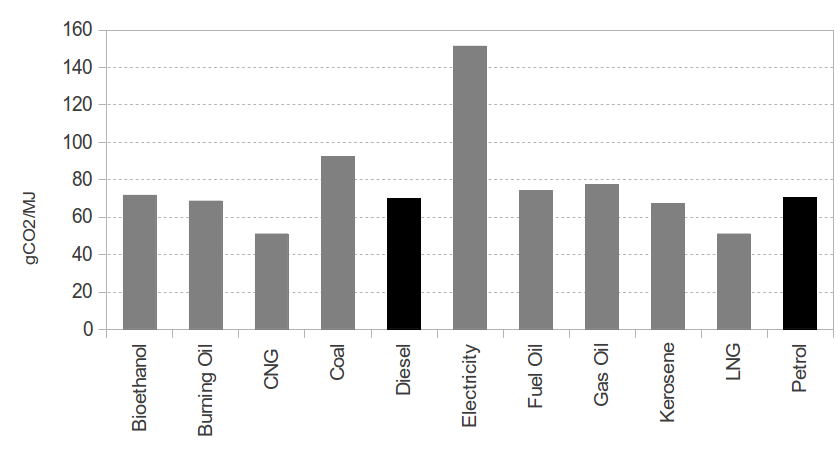
\includegraphics[width = 12 cm]{gco2}}
  \caption[The greenhouse gas emissions per unit energy of various fuels]
{The greenhouse gas emissions per unit energy of various fuels. Data
taken from \citet{Defra2011} (additional sources for
\href{http://www.ipcc.ch/pdf/special-reports/sroc/Tables/t0305.pdf}{\color{blue}electricity}
and
\href{http://www.biomassenergycentre.org.uk/portal/page?_pageid=75,163182&_dad=portal&_schema=PORTAL}{\color{blue}biofuel}
emissions were used)
and converted into SI units. The dominant
transport fuels are black for emphasis.  }
  \label{fgco2}
\end{figure}

The reasons for advocating a focus on energy use,
and not emissions directly, can be summarised as follows:
\begin{itemize}
 \item Emissions can be variable depending on the energy/fuel source, whereas
 energy is constant across fuel sources.
 \item If energy use is reduced overall, carbon-intensive forms can be phased out.
However, if emissions from one sector fall, they may well rise in another as
fossil energy resources are freed-up.\footnote{For
example, imagine if transport emissions rapidly dropped to zero
due to electrification and rapid uptake of renewables. The additional
load on the grid caused by this new user \citep{dyke2010impact} could
lead to an increase in the emissions stemming from space heating because
the total supply of renewable energy is fundamentally
limited by the laws of physics \citep{MacKay2009}. \citet{Berners-Lee2013}
describe this problem with emission reduction plans overall as squeezing
a balloon: savings in one area tend to bulge out in another.}
 \item Energy is the `master resource' from which all others (including more
energy) can be obtained; emissions are the end result result of energy use.
 \item It can be argued that energy use is at the root of the linked `big picture'
problems mentioned in this chapter, not just climate change. Therefore
tackling the energy problem could have numerous co-benefits.
\end{itemize}
All this suggests that the climate debate should be much more closely
linked to the energy debate. Specifically, the carbon content of proven
fuel reserves should be compared with the carbon dioxide content that
can safely be burned. Doing this analysis, based on recently released
data on fossil fuel assets, has led to an alarming finding: ``for all the
talk about finite resources and peak oil, scarcity is resoundingly not the
problem. From the climate's perspective, there is far too much fossil fuel''
\citep[p.~29]{Berners-Lee2013}.
% In fact, to keep the chances of a
% global temperature increase below two degrees centigrade
% (the point beyond which many studies show would be dangerous),
% above 75\%, \citet{Berners-Lee2013} showed that humanity can burn only
% around a half of economically viable reserves.
\citet{Berners-Lee2013} show that for there to be at least a 75\% chance
that the global temperature increase remains below two degrees humanity can
burn only around a half of economically viable reserves.
In terms of personal transport, this means
phasing out petrol and diesel and avoiding carbon-intensive electricity sources:
a fundamental shift.

Most greenhouse gas emissions stem from burning fossil fuel use, and once
extracted, these fuels are invariably burned. This has led to the conclusion
amongst some that the solution must be top-down:
fossil fuel companies must be forced to leave most of their assets untapped.
This can be achieved 
either through plummeting prices of fossil fuels or through regulation.
The former case is currently highly unlikely due to the surge of fuel demand from
emerging economies, combined with the sheer utility of fossil
fuels.\footnote{However,
if governments, in coordination,
prioritise minimising energy use while maximising
uptake of renewable energy, the former possibility would become more feasible.
}
The latter also seems unlikely, following the failure of UN talks in
Copenhagen to arrive at a consensus on legally binding
and enforceable emission targets for the major emitter.
This research is relevant in any case: if fuel prices remain high there
is a strong economic incentive to reduce energy imports. If leaders worldwide
agree to tackle climate change through top-down or bottom-up
policies, there will clearly be a strong interest in how best to
reduce reliance on fossil fuels in every sector that is vital for
well-being. Regardless of the level of regulation (whether it
occurs at the point of extraction or use of fuel), it implies high consumer prices
for fuels, through policies such as taxes, a
`carbon cap' or even energy rationing.\footnote{Interestingly, high prices of fossil
fuels is also the end result of many scenarios of resource depletion, which
has historically been another major driver of research into energy and
transport \citep{Fels1973}.}
% At this stage, it is worth noting that some people,
% including a number of politicians, believe that
% anthropogenic climate change should not be a political priority. Climate
% contrarians, some funded by the fossil fuel industry itself,
% have managed to confuse large sections of the public.
Another pragmatic benefit of the energy approach is that even if one questions
the need to tackle climate change, the arguments to reduce dependence on
finite fossil fuels for other reasons are very strong.

\subsection{Peak oil and resource depletion}
On addition to the impacts of climate change,
depletion of our fossil energy resources is another non-negotiable
reason for transition away from fossil fuels, to a ``post-carbon'' economy
\citep{Heinberg2005, Heinberg2009, Heinberg2010, Kunstler2006}.
Oil is the most rapidly depleting resource yet motorised
transport is almost entirely dependent on liquid fossil fuels
derived from it \citep{Gilbert2008}.
Multinational personal transport industries tend to downplay or deny the risks
of peak oil, pointing to non-conventional oil resources and technological
advance as reasons not to worry. Prototype biofuels, electric cars and hydrogen
fuel cells are often cited as ways of overcoming high prices. This is ironic
because each technology is highly dependent on oil for resource extraction,
manufacture, distribution and waste disposal stages of their life-cycle: high
oil prices could make the batteries for electric cars, to take one example, even more
expensive, far out of the reach of the median global citizen.
%!!! income?
Each technology is still in the research phase of development,
relies on scarce public subsidies to be commercially viable and cannot operate
on the scale needed within modern transport infrastructures even if production
lines producing them were scaled up before a major oil shock. Biofuels, to take
the most heavily subsidised example, can only ever produce a small fraction of
current transport energy demand even if all available resources were exploited
to the maximum (\cref{f:biofools}).

 \begin{figure}[htbp]
  \centerline{
    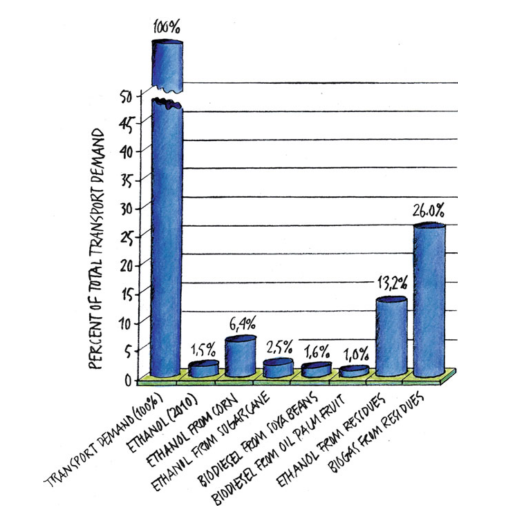
\includegraphics[width = 12 cm]{biofuels-cont}}
  \caption[Biofuels' contribution to global transportation energy use]
{Biofuels' current (2010) and potential contribution to
global transportation energy use \citep[p.~228]{Aleklett2012-peeking}.
Image used with permission of author. Data originally presented in
\citet{Johansson2010-ag-fuel+food}.}
  \label{f:biofools}
\end{figure}


For this reason peak oil is a major motivation for research into energy and
transport. How will transport systems operate beyond 2050,
when oil production will be a fraction of its current level? 
\citep{Aftabuzzaman2011}.
How will people get to work in the event of shortages?
\citep{Noland2006}. These are just a couple of examples of
the kinds of questions that are being asked in preparation for
declining oil supply. A parallel question
(explored in \cref{svul}) is: how will commuters be affected by
oil price shocks, depending on where they live and their socio-demographic
characteristics? The potential problems posed
by peak oil for motorised transport systems are severe and include
collapse of complex economic activity due to the
highly inter-dependent nature of the global economy \citep{Friedrichs2010,
Korowicz2011}.
For this reason an introduction to peak oil, and how it relates
to commuting, will help to place this research in the wider
context. \citet{Gilbert2008} provide a comprehensive reference
on the subject, from a North American perspective.

Peak oil is the point at which global oil production
enters terminal decline due to depletion of large oil fields
\citep{Greer2008}. It is an inevitable event during the 21$^{st}$
century, as oil is a finite resource, approximately half of which
has been used \citep{Aleklett2010}. However, there remains controversy
about the exact timing of the peak \citep{Smil2008}.
An in-depth review by the UK's Energy Research Centre \citep{UKERC2009}
found that the weight of evidence suggests a peak in the near-term,
before 2030. This is
well before the 20 years that the famous Hirsh Report \citep{Hirsch2005}
indicated would be needed to prepare for declining supplies of liquid fuel.
The implications are stark: if peak oil does occur before 2030, as
the evidence reviewed by \citet{UKERC2009} suggests, urgent preparations
must begin now.

As economists have long indicated \citep{Solow1974},
it is not only the amount of oil left in the ground
that directly affects peoples' lives. It is the \emph{price} of oil that
affects transport systems, with knock-on impacts on human lives.
Price is also affected by changes in demand and technologies for
extraction and substitution \citep{Perman2003}.
Over the past decade there has been increasing evidence that depletion
plays a major role in determining global oil prices, however,
with high and volatile prices likely in the future \citep{Aleklett2012-peeking}.
The price of crude oil during the past 20 years has shown both volatility
and (when a smoothed by a rolling average function) a near inexorable
upward trend \cref{fig:oilprice}. 


 \begin{figure}[htbp]
  \centerline{
    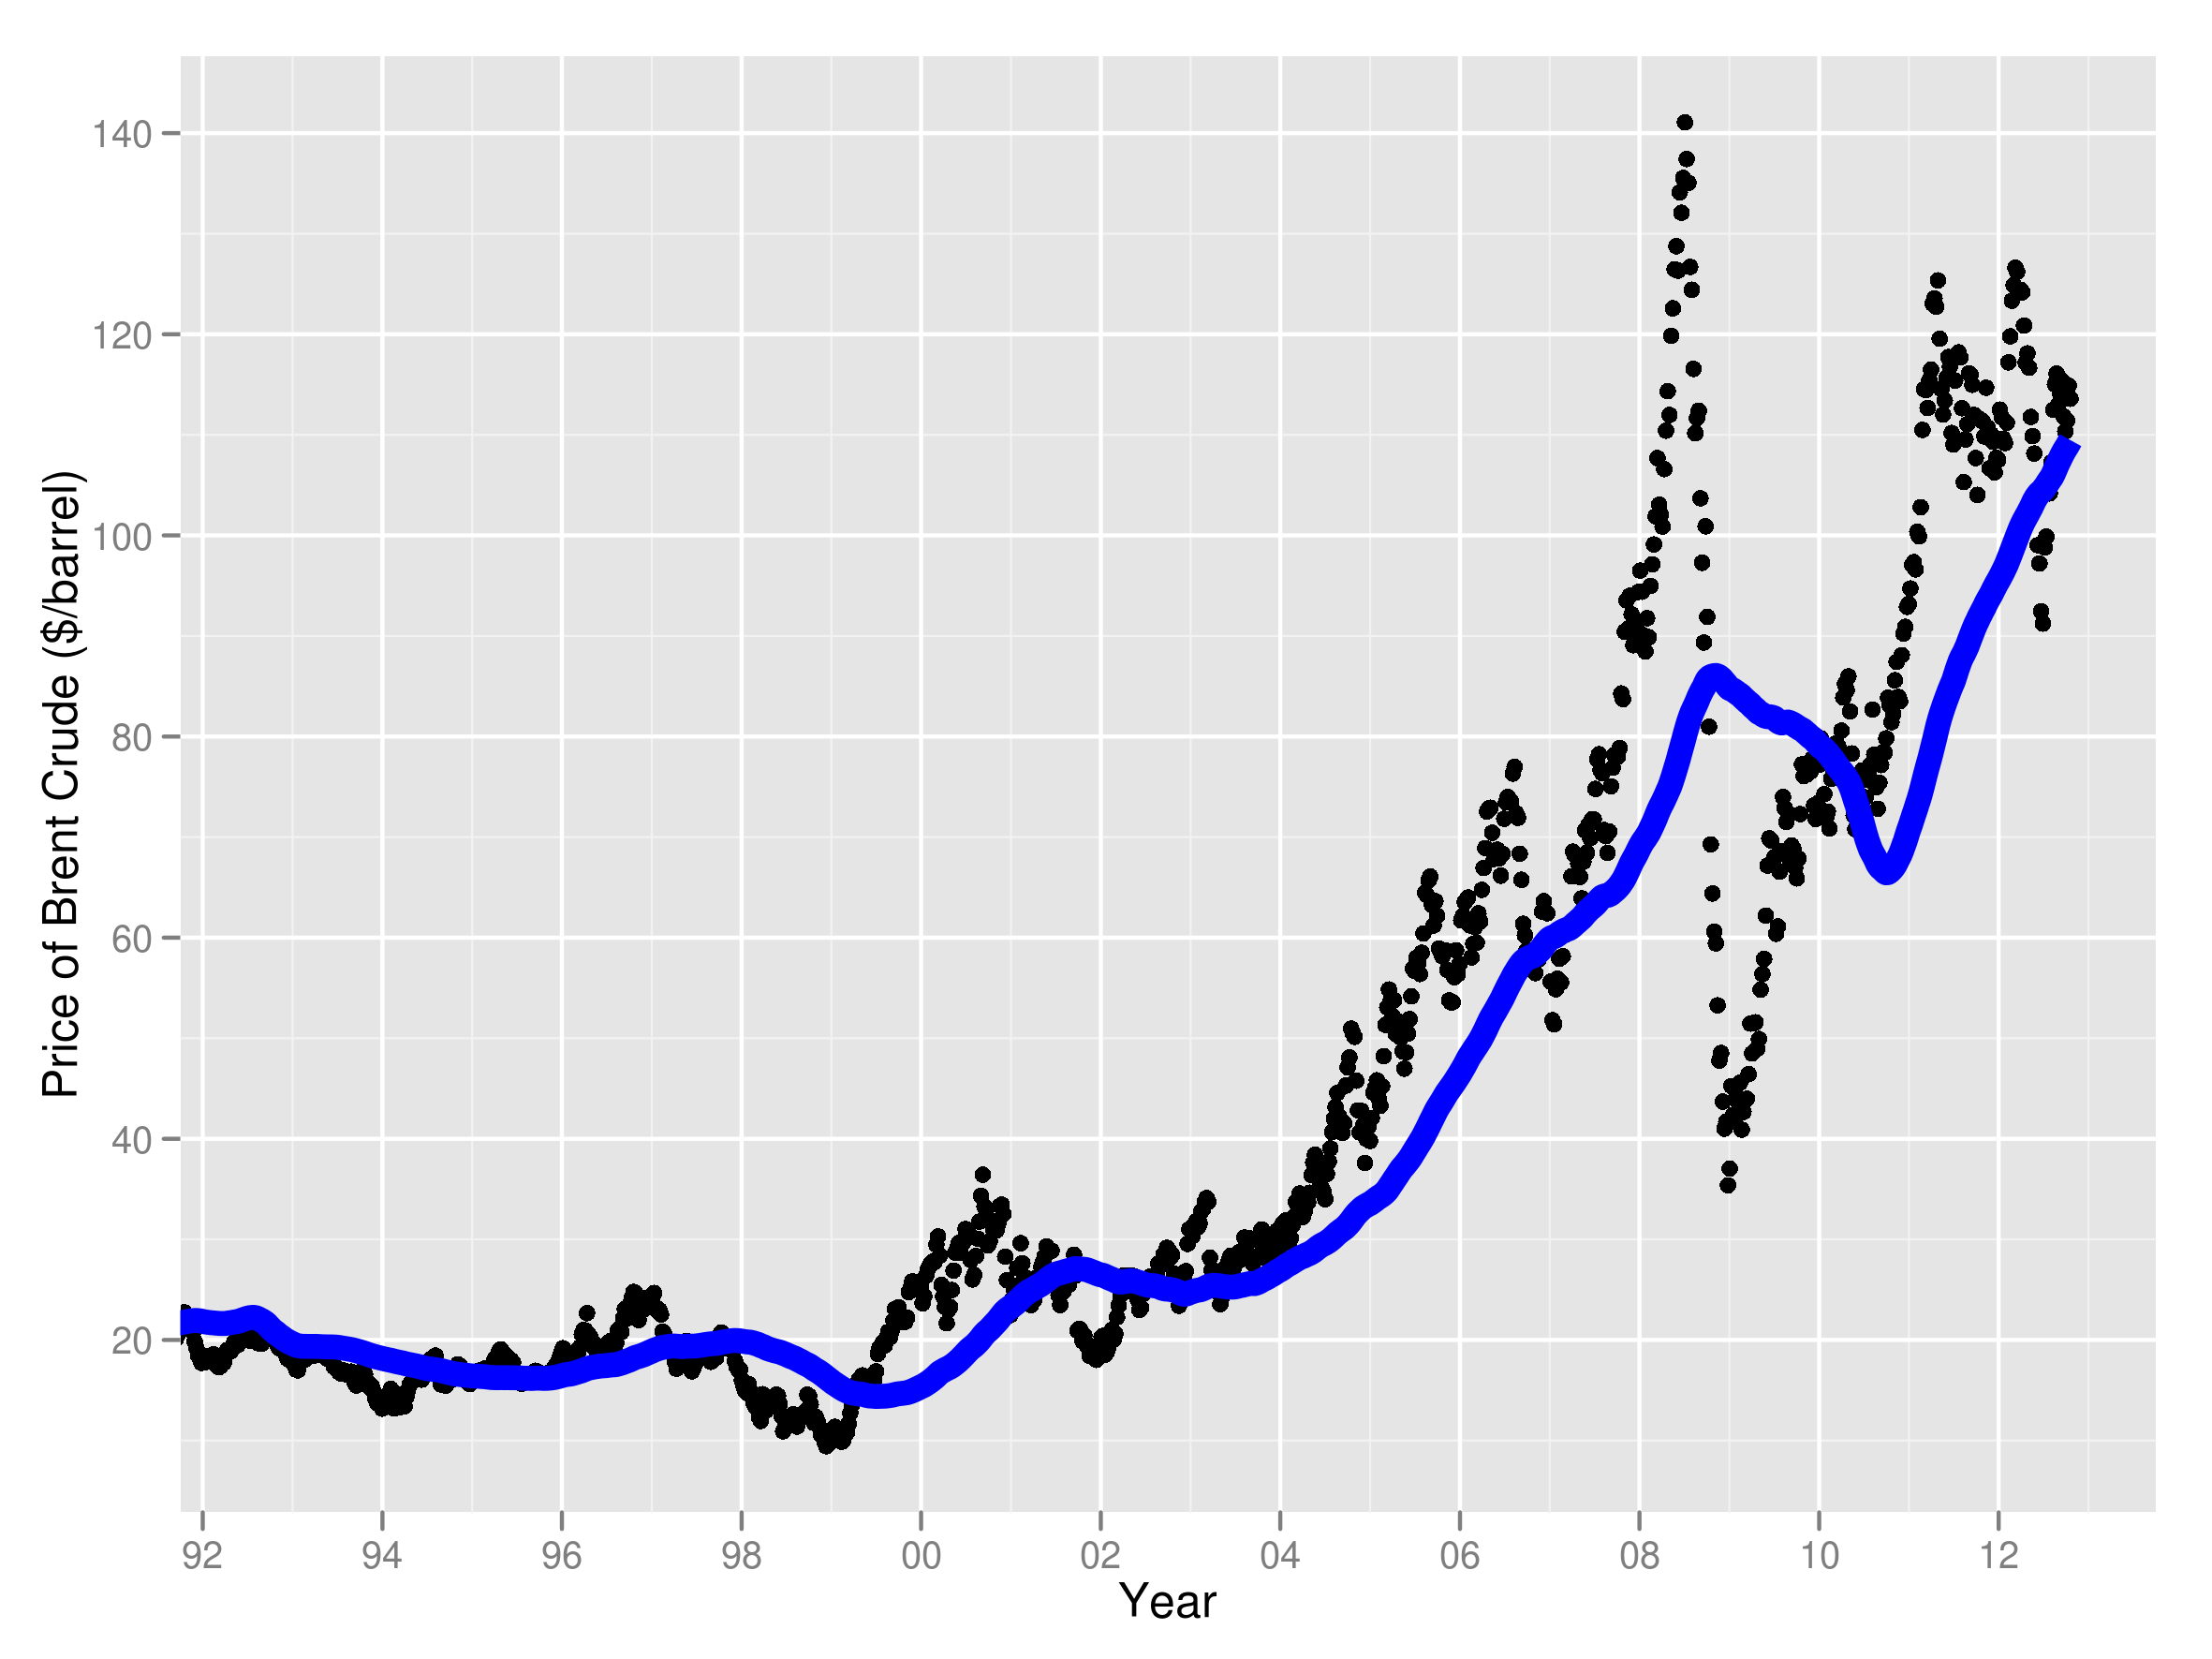
\includegraphics[width = 12 cm]{oilprices}}
    \rule{35em}{0.5pt}
  \caption[Average prices of Brent Crude oil spot prices, 1992 -- 2012]
  {Average prices of Brent Crude oil spot prices per week,
January 1992 until October 2012 (dots) and a 2 year rolling average
(blue line) Data from the U.S.~Energy
Administration (\url{http://www.eia.gov/dnav/pet/pet_pri_spt_s1_d.htm})
plotted using the R package ggplot2.}
  \label{fig:oilprice}
\end{figure}

Despite these upward trends, UK government energy policies
are still largely based on the assumption that oil prices will
remain below \$100 per barrel into the 2020s \citep{UKERC2010}.
Thus methods that estimate the oil-reliance of households based
on readily available commuter statistics could be highly relevant
to politicians and planners making long-term decisions. The ability to
quantitatively explore
the impact of high oil prices and other scenarios of change
at the individual level is an output of this
research that could have applications in transport policy evaluation and 
development. See \cref{Chapter7}.

\subsection{Inequality and well-being}
Peak oil and climate change are important because we
depend on the resources and processes of the natural environment to survive.
Humans also depend on the relationships between each other, not simply for
survival, but for quality of life. ``It is only in the backward countries of
the world'', wrote John Stuart Mill, ``that increased production is an
important object; in those most advanced, what is needed is a better
distribution'' (Mill 1857, in \citealt{Perman2003}: p. 6).

With more than 150 years of hindsight, Mill's statement seems all but
Utopian: economic growth is still the number one priority of most governments
worldwide, even in wealthy countries such as the UK where evidence
suggests that further growth may do more harm than good, for people and
the environment \citep{Latouche2008}.
To such an extent does economic growth dominate modern decision making,
regardless of consideration of how growth is distributed,
that authors such as Charles Eisenstein and John Michael Greer
refer to it as the founding story of our age \citep{Eisenstein2011, Greer2009}.
In contrast to this dogmatic growth focus, evidence suggests that
other things, including equality of economic and social opportunities, lead
to quality of life \citep{Jackson2008, Jackson2009}.

The growth-at-all-costs mentality, combined with our debt-based
capitalist economy\footnote{As explained by \citet{Eisenstein2011},
the very existence of positive interest rates ensures that those who
have money tend to have more. According to this view, growing
levels of economic inequality is built into the monetary system,
and can only revert back to low levels with crises such as
wars or depressions, planned debt annulments or
(preferably for Eisenstein) negative interest rates.}
has caused inequalities to grow worldwide
\citep{OECD2011}. The UK has one of the highest levels of
inequality in Europe (\cref{fig:ineqs}).

\begin{figure}[htbp]
  \centerline{
    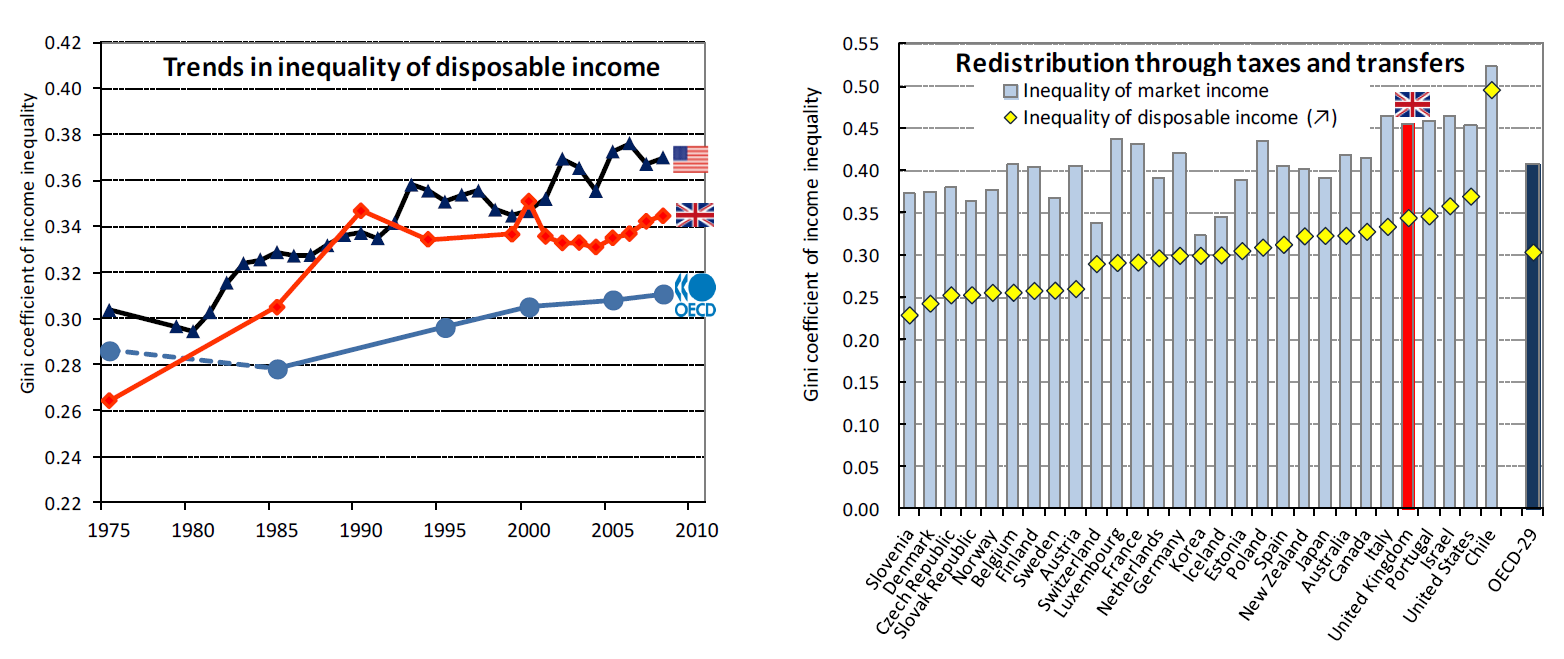
\includegraphics[width = 15 cm]{oecd}}
    \rule{35em}{0.5pt}
  \caption{UK Gini index for market and disposable income
  in context \citep{OECD2011}.}
  \label{fig:ineqs}
\end{figure}

This problem is important in the context of the energy costs
of commuting because employment opportunities are greatly
affected by one's ability to find and affordably travel to work.
Variable transport opportunities amplify social and economic
inequalities: 38\% of jobseekers say transport problems prevent
them from getting a job \citep{SocialExclusionUnit2002}⁠.  ``No jobs nearby'' and
``lack of personal transport'' were the first and second most
frequently cited barriers to getting or keeping a job in a survey
of young people in the UK \citep{Bryson2000a}⁠.

% \subsubsection*{Well-being}
% \label{s:well}
% In addition to the readily quantifiable impacts of commuting on climate change,
% rates of non-renewable resource depletion and (to a lesser extent) economic
% opportunities and inequality, the daily trip to work also has a direct impact
% on well-being. This body of literature can be divided into three main areas:
% commuting and physical health, psychological impacts and how the impacts
% of commuting vary between people, for example based on gender and class.
% Key papers in each of these areas are highlighted below.
% 
% Commuting involves a substantial amount of time, effort and expenditure. It
% is (for the xx\% of employed people in Britain who do not work at home)
% an essential component of daily economic life which.
% It is worth, at this stage, reflecting briefly on employment because if
% employment is an optional extra, the well-being impacts of commuting could
% simply be avoided by not working. However work appears to be integral
% to well-being for most adults.
Paid employment, and the
economic independence it brings, is a foundation for life satisfaction
\citep{Jahoda1982}. Work is ``a principal source of identity for most adults''
\citep{Tausig1999} and can promote good health (if the work is satisfying)
\citep{Graetz1993}. By corollary unemployment, the proportion of working-aged
people without a proper job, ``is a crucial indicator of the welfare and
economic performance of different areas'' \citep[141]{Coombes1982}. Yet without
accessible means of travelling to and from work each day, these benefits are
impossible to reach.

Given the importance of work, and the high proportion of work that is
undertaken outside the home, it should come as no surprise that
people will commute even if it an arduous task damaging to their health.
Taking a broad definition of health, these impacts range from those
narrowly associated with breathing urban air to more subjective consequences for
mental health including stress. From a human ecology perspective
commuting can be understood as a stressful relocation from one's
`domestic habitat' to a more hostile, hierarchical workplace. %%%%% ref!!!
The trip to get there will often coincide with thousands of other
commuters, all using the same road, railway or path. With these factors
in mind, the finding that, ``For most people,
commuting is a mental and physical burden'' should come as little surprise
\citep{Stutzer2007}.\footnote{The question
``how much of a burden'' is open to debate, however.
The finding of \citet{Stutzer2008}, that subjective well-being
declines proportionally with time, was not replicated in a
recent analysis of data from the BHPS \citep{Mumford2012}.}
The entrenched issue of inequality is tackled from
the perspective of commuting by measuring it in energy
(as opposed to purely monetary) terms (\cref{sindvar}) and providing
methods for assessing the distributional impacts of future
what-if scenarios (\cref{Chapter7} and \cref{Chapter8}).

% \subsection{Why energy?}
% The 

\section{Commuter energy use: everyday realities}
\label{s:realities}
The large scale processes of change mentioned above tend to be thought of in the
abstract, using inevitably simplified versions of reality. They are
often best represented through statistics, inherently simplified and
aggregated for visualisation. Seeing the issues quantitatively and
at `arms length' may be necessary to
gain an objective understanding of their evolution. Yet this may also lead to lack
of understanding of their local-level manifestations and poor retention in memory:
although physical
reality may be best understood through numbers, human brains seem better able to
retain information that has emotional or personal content
\citep{Laird1982, Green2012}.
% \footnote{This enhanced recall for emotional information
% appears to be linked to emotional sensitivity in general
% which is generally higher for women:
% ``An individual’s level of emotional sensitivity
% was a stronger predictor of their emotional recall
% than their gender, suggesting that memory for
% emotional information is not determined by
% gender alone, but instead reflects a person’s
% sensitivity to emotional information in their
% environment. Thus, gender differences in memory
% for emotional information observed in the present
% study most likely reflect that women are, on
% average, more sensitive than men to the emotional
% aspects of their environment''
% \citep[p.~204]{Bloise2007}.
% }
When explaining my research to others, the following question
has been found to
effectively transform a purely academic and boring issue into something
interesting and relevant:
``What would a doubling of global oil prices mean for your family?''
For this reason, and to introduce some themes that
are used throughout this thesis in `layman's terms', this section is
based on a brief personal story: that of Chris Fisher.

Chris was born and bred in Weobley, a small town nestled between Hereford,
Leominster and Kington (\cref{fig:hereford}). Since finishing
at Weobley secondary school he has worked in a
wide range of jobs in the local area, including for Weobley's largest employer
(and sponsor of the village football team) Primasil and a local restaurant
called Joules. His current job, held for over 3 years now, is
to provide manual labour in Tyrrell's crisp factory.

\begin{figure}[htbp]
  \centerline{
    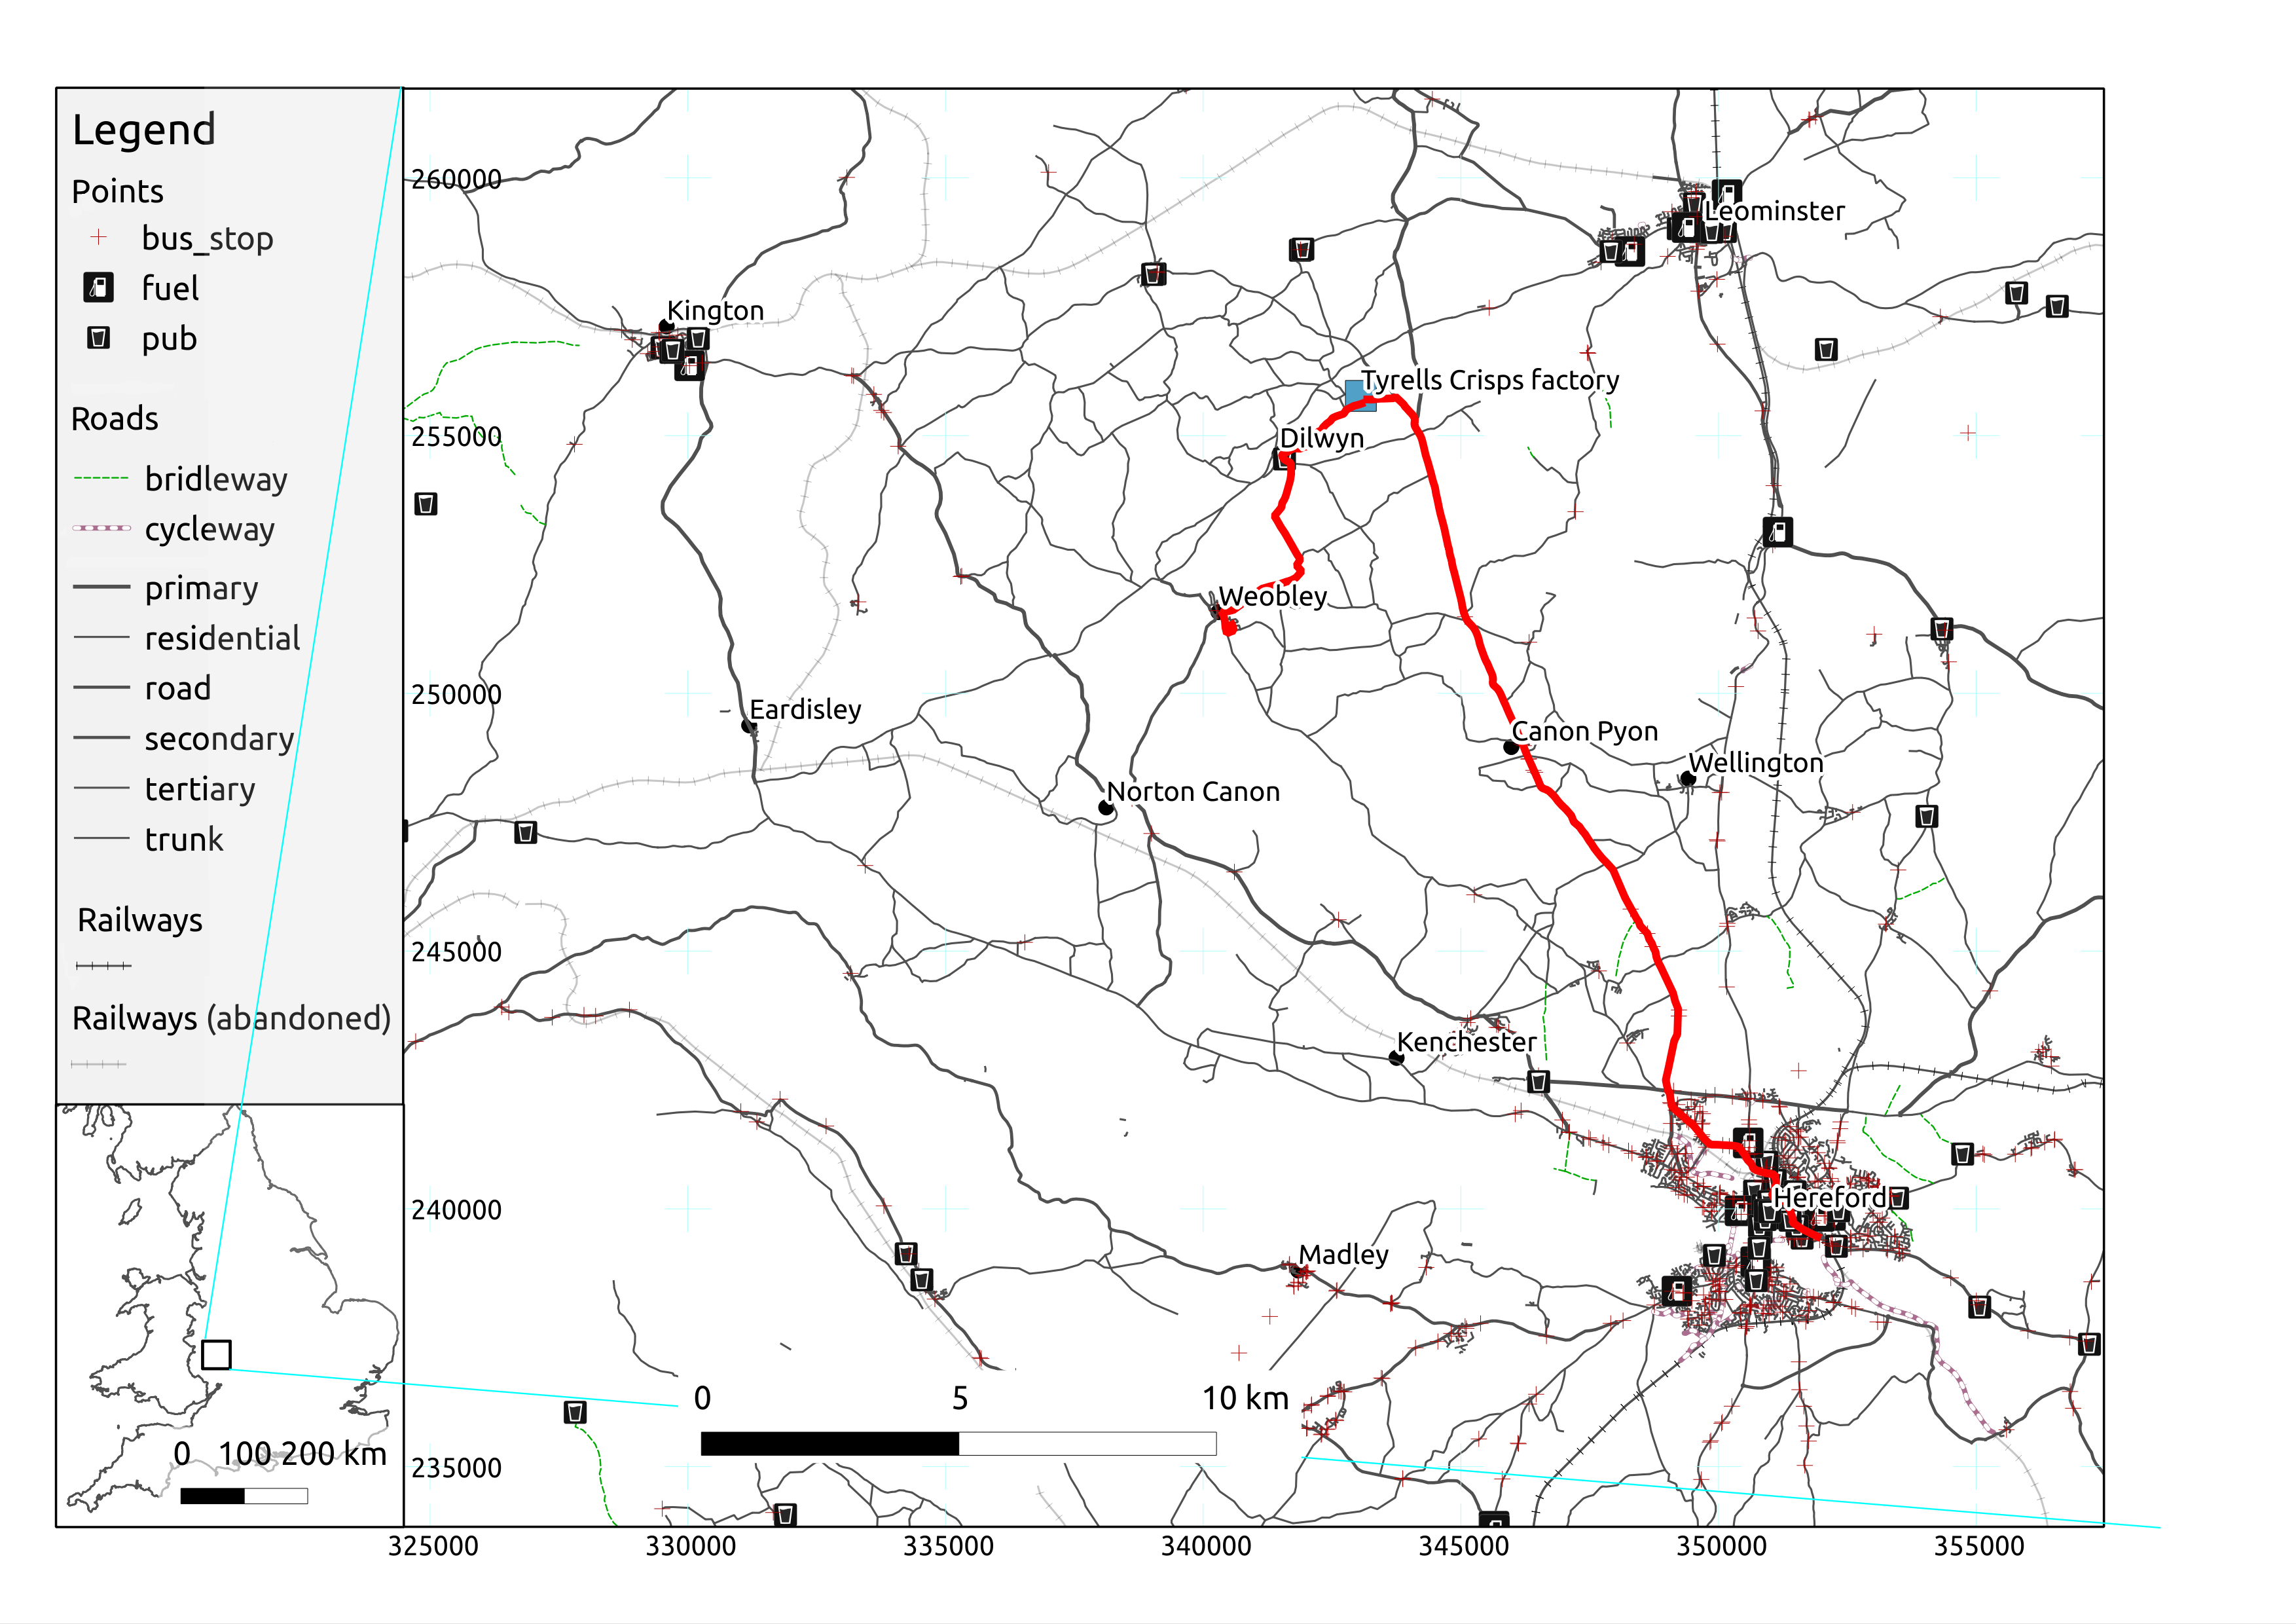
\includegraphics[width = 16 cm]{hnew}}
    \rule{35em}{0.5pt}
  \caption[Commuting options to Tyrrell's crisp factory]{Commuting options to
Tyrrell's crisp factory for Chris Fisher if he lives in Weobley (7 km one way)
or Hereford (13 km one way), as illustrated by the thick red lines.}
  \label{fig:hereford}
\end{figure}

Commuting and the economic cost it exacts has a large impact on Chris's life.
Ideally he would like to move to Hereford as that is where more of his
friends live and because there is more going on in the city than in Weobley.
However, Chris feels
bound to continue living with his mum in Weobley due to the costs of commuting.
The numbers work out like this: it's an 8 to 9 mile round trip to work from
Weobley, whereas the distance would approximately double if he lived in Hereford.
The location of his job also essentially forces car ownership: there are no buses
between Weobley and the Tyrrell's crisp factory, car sharing options are limited
and relying on a bicycle does not seem feasible for winter shifts that end at 6 am.
In addition to location, other downsides include long hours (12 hour shifts for
everyone, 4 days on, 4 days off), poor pay (\pounds8 per hour) and unpleasant
working conditions (the factory contains no windows, meaning that during
some day shifts you do not see the sun for 4 days in a row). For these reasons
Chris was tempted to quit when Tyrrell's decided to move towards 24 hour
production following increased demand from the USA: previous to this change
8 hour shifts were the norm; afterwards 12 hour shifts were implemented, broken up by
three 20 minute breaks.
% \footnote{This industrial regime is ironic given that
% part of Tyrrell's appeal is their `local' feel: on the company's website this is
% hammered home in the following blurb:
% 
% ``We're proud Herefordshirians [sic]
% (is that a word?), so we only use potatoes
% from local farmers, our favourites being Lady Rosetta and Lady Claire.
% They're the names of the potatoes, not the farmers.
% Just to be clear.''
% 
% In contrast to this artisan advertising, the management seem
% to treat the local employees as cheap labour rather than a treasured and
% unique group of people. For example, wage rises were promised following the
% implementation of 12 hour shifts but 6 months after the salary remains
% fixed at \pounds8 per hour, this time with no prospect of earning overtime.
% }


Despite these issues Chris has so far
decided to stay on at Tyrell's because
``if you live in Weobley, there are not many jobs.''
This context is important, because it illustrates how commuting
interacts with everyday life dilemmas, in this case
between moving house or staying put and
between quitting an exploitative job or finding a new one.
Ideally, Chris would like to sell his car, get a job in Hereford and be able
to walk to work each day. However, he's adapted to the new shifts, and
enjoys the 4 days of freedom he is allocated out of every 8, using them
to climb mountains, go to gigs and relax. The need to own a car
(on which 20\% of his income goes) and the expenditure on commuting
(5 to 10\% of his income) are disadvantages that can be endured for now.

Chris almost always drives to work. He has cycled a few times in nice weather
and would like to cycle to work more frequently. However, the
prospects for \emph{modal shift} are not great at present: his bike is not
much good, and the prospect of cycling 5-odd miles at 6 in the morning
after a physically punishing 12 hour shift is not attractive.
Chris is very interested in the cycle to work scheme, and believes he
would cycle more if he had a decent bike --- a friend was able to
get a \pounds900 bicycle through them. That's the semi-solution that
will be pursued in the short-term, and that goes well with Chris's
fitness hobbies.
When asked about the impact of the commute on his quality of life
Chris gave a short answer: ``not a lot really.'' For him commuting
is simply a means to an end --- to get to paid employment --- which
in itself is just a way to earn a living.

The sheer complexity of commuting on a national scale is well illustrated
by considering that Chris's commuting behaviour, plans and experiences
are just one data point out of hundreds of thousands. Subtleties of
his current behaviour,
% \footnote{For example he occasionally cycles and lived `car free'
% during 7 months last year.
% }
let alone the transient nature of his working
hours, shift patterns, home location and employment status are not
picked up by questions in the census or, to varying degrees, in the
national travel surveys (see \cref{Chapter4}). Nevertheless, the things that
Chris allocated importance to --- the distance to work, the time and money
costs of the commute and the availability of alternative modes --- indicate
that quantitative analysis of these aspects of the problem
of commuting is appropriate and relevant to everyday life.

There are certainly many unknown and highly varied individual circumstances,
such as Chris's that can never be squeezed into simple numerical models.
However, the variables about which good geographical data are available
(mode and distance) and the variables which can be calculated
with varying levels of uncertainty (e.g.~economic costs,
potential for modal shift), match the factors that held most
sway for Chris, with the exception of the location of his friends.
% \footnote{Even this could in theory be estimated, based on central place theory.}

% \section{Commuting as a global phenomenon (dodgy)}
% Chris Fisher's experience illustrates the importance of distance,
% available modes of travel and economics in the humble journey to work for one
% individual. On the global scale, commuting is vast. It is a near ubiquitous
% indicator of a formal economy, and consumes huge
% amounts of time, resources, and money (fig. on country commuter distances
% would be mint here). A `back of the envelope' calculation suggests that ~ xxx TJ
% of primary energy are consumed worldwide during 2 billion daily commuter trips,
% excluding indirect energy costs such as vehicle production, fossil fuel
% extraction, and road maintenance.\footnote{
% %
% Add method here
% %
% }
%  To provide a sense of scale, this translates to 2\% of global primary energy
% use (xx EJ) and 4\% of oil consumption across the globe. Commuting is also
% complex, taking place in myriad contexts
% and by a plethora of different modes. Charcoal burners... ,
% Factory workers in ..., The challenges faced by Chris Fisher regarding his  8
% mile car trip to the Tyrrel's crisp factory in Herefordshire may not be
% representative of commuting worldwide, but its importance in everyday life and
% the problems it poses for welfare and sustainability found everywhere.
% 
% To reiterate, journeys to work are dynamic and
% diverse: their \emph{length}, \emph{mode}, and \emph{costs} vary depend on a
% range of range of factors that also change over time and space. These are the
% fundamental characteristics of commuting and the building blocks of this
% research. These three variables also determine another important characteristic
% of commuter trips: their energy costs. This abstract yet quantifiable variable,
% based in physical reality, is increasingly important in a world of emissions
% targets, environmental awareness, and depleting oil fields. A review of previous
% work on commuting indicates that its quantification is also often absent
% in transport and energy policy. For this reason the energy costs of transport to
% work is the main concern of this PhD: understanding its variability across
% space, time and between people and interpretting what these results may mean
% for future transport policies is the broad goal. Each section of this
% thesis contributes to this goal. Before describing the contribution of each
% chapter, it is important to understand a little about the case study region,
% and why it was chosen.
% 
% Could include section on Getting to work in a 'post carbon' future here.

\section{The importance of commuting} \label{snimportance}
The previous two sections have illustrated the importance of commuting
in terms of its impact at the individual level,
and in the global context. In many countries, however, the importance of
commuting can be investigated using a more detailed source of information:
national transport statistics. This section introduces
aggregate level travel to work statistics from the UK Census,
which form the foundation of analysis in the coming sections, and outlines
the variability of commuting patterns nationally.
Based on these statistics, it also illustrates the importance of
commuting in comparison with other reasons for travel.

% These statistics demonstrate that there is no single way to measure the relative
% importance of travel to work compared with other reasons for personal travel
% such as shopping and `the school run'.
% 
% The relative importance of commuting
% as a reason for trip will depend on how you value personal travel, whether number
% of trips, distance, time or energy use are considered as appropriate measures
% of ``importance'', or what constitutes `essential' travel.
% Do I mention each of these points?

% Overall, commuter flow data tends to be the most reliable
% source of personal travel statistics. This is because
% travel to work is regular and predictable in time and over space.
% Distance can also be estimated quickly, based only on matched
% home-work postcodes.

% These, and other defining characteristics of work travel such as
% rates of occupancy and  multi-purpose trips are also explored, towards the
% sections end. These national-level data, placed in context, help to introduce
% commuting as a unique and important trip type and outline gaps in our knowledge.

\subsection{Trips}
Trips are the basic unit of travel, ``a one-way course of travel
with a single main purpose'' \citep[p.~6]{Dft2011-notes}. The data presented in
\cref{fig:trip-nums-gb} (and henceforth)
therefore counts the daily journey to work and
back as two trips. The value for commuting provided by this dataset
(150 trips per year) may therefore
seem surprisingly low, implying that people only work an average of 75 days per year
--- \citet{hall2011tourism} estimate that roughly
400 commuter two-way trips are made per capita
per year worldwide. However,
the National Travel Survey samples all citizens, including children and the
elderly; the average number of trips made by commuters --- the focus in this
thesis --- is estimated to be double this figure, around 320 (\cref{sfreq}).

\begin{figure}[htbp]
  \centerline{
    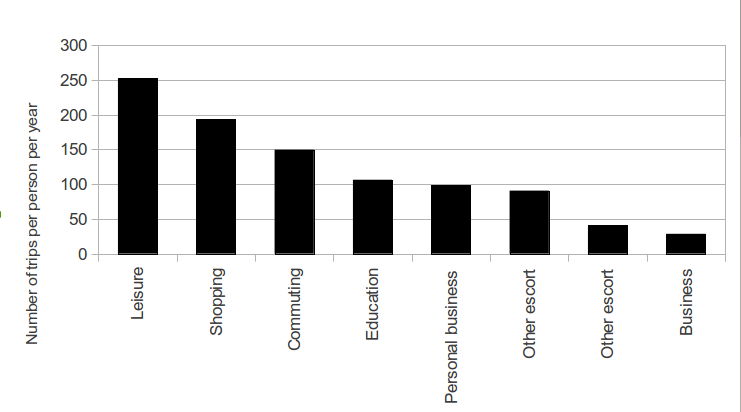
\includegraphics[width = 14 cm]{./Figures/trip-nums-gb}}
    \rule{35em}{0.5pt}
  \caption{Average number of trips per person per year across Great Britain.}
  \label{fig:trip-nums-gb}
\end{figure}

\subsection{Distance}
% The total distance of trips made by each trip type is equal to the number of
% trips made, multiplied by the average distance. Commuter trips averaged 14.2 km
% in 2009/10, slightly longer than the average trip distance for all trips Great
% Britain (11.3 km). Commuter trips are the third longest type of trips in the
% UK, following holiday and business trips, whose average values are greatly
% increased by flying. %Dad'd
The distance made by all trips is their number multiplied by their average distance.
Commuter trips averaged 14.2 km in 2009/10, slightly longer than the 11.3 km
average for all trips in Great Britain and the third longest,
following holiday and business trips. The average length of the latter
are greatly increased by flying.
This information
% , as well as the evolution over time,
are illustrated in \cref{fig:dist-trip-gb}.

\begin{figure}[htbp]
  \centerline{
    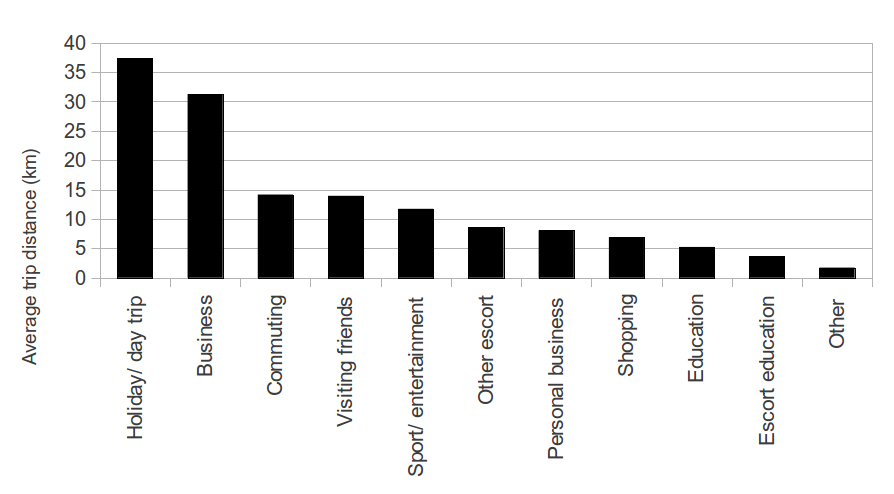
\includegraphics[width = 14 cm]{./Figures/dist-trip-gb}}
    \rule{35em}{0.5pt}
  \caption{Average trip length by purpose in Great Britain.}
  \label{fig:dist-trip-gb}
\end{figure}

The average distance of each trip helps characterise commuting as relatively
long-distance compared with other trip purposes such as shopping (6.9 km).
However, total travel distance is more important from an energy perspective:
long leisure trips, for example, are comparatively unimportant in energy terms if
they are infrequent. The data shows that leisure travel\footnote{Leisure
trips include holidays and social trips, in the 2010 National Travel
Survey \citep{Dft2011-notes}.} dominates trip distances, despite the sporadic
nature of international holidays. Commuting is in second place, responsible for
2160 km of personal travel each year for UK citizens, including those under 16.
For commuters, the average total distance of commute would be approximately
double this value (\cref{fig:dist-purp-gb}).

\begin{figure}[htbp]
  \centerline{
    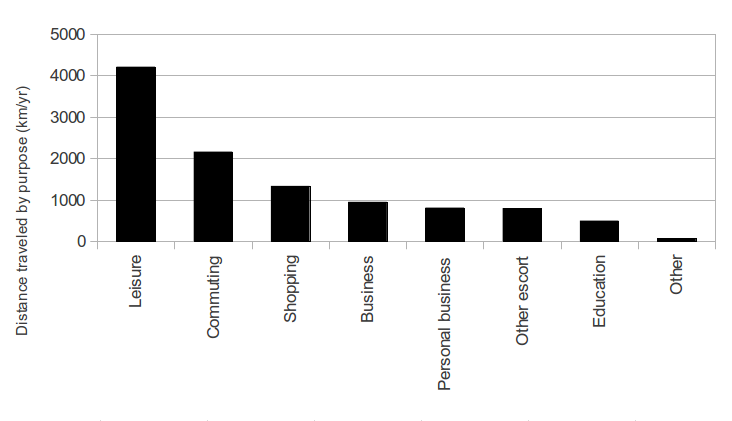
\includegraphics[width = 14 cm]{./Figures/dist-purp-gb}}
    \rule{35em}{0.5pt}
  \caption{Total distance travelled by mode in Great Britain.}
  \label{fig:dist-purp-gb}
\end{figure}

\subsection{Time}
\index{trip duration}
From the commuter's perspective, the number and distance of commuter trips made
may seem relatively unimportant: in the formal economy, time is money and
people are increasingly rushed to face up to professional and family
commitments \citep{Eisenstein2011}. Therefore, time is another measure of importance that
should receive attention in any introduction to commuting. Overall commuting is
the the most time-consuming reason for personal travel in the UK, accounting
for 19\% of trip time, consuming 70 hours per year. Because both the numerator
and the denominator in this measure (hours per year) have time units, travel to
work can also be presented as the percentage of one's life spent travelling to
and from work\footnote{This
is a potentially poignant metric for those who
spend more than 5 hours per working day or more than 10\% of their life simply
getting to work and then turning around going home again!}
(\cref{fig:t-commuting}).

\begin{figure}[htbp]
  \centerline{
    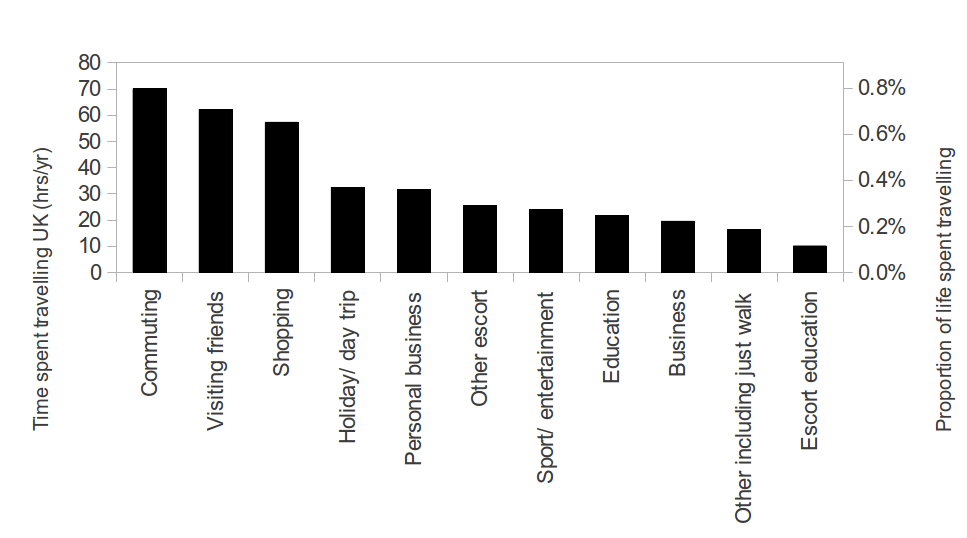
\includegraphics[width = 14 cm]{./Figures/time-commuting}}
    \rule{35em}{0.5pt}
  \caption[Time spent commuting in Great Britain]{The average time spent by
citizens of Great Britain travelling to work and back each year. The right hand
axis illustrates the same information, this time as a proportion (data
source: \citealp{NTS2012-time-travel}).}
  \label{fig:t-commuting}
\end{figure}

There is pronounced regional variation in the average time spent travelling to
work. This variation is linked to the average time per commuter trip (high
total work travel time values are influenced by how frequently people work),
the distance to workplace, and, of prime importance, levels of congestion.
% (\cref{fig:really?}).

% \subsection{Energy} % Include this!
% The energy costs of commuting is a complex subject with variability over
% time, space and from person-to-person. However, its relative importance
% compared with other sectors of the economy can be estimated rapidly,
% using simple `back of the envelope' calculations. 

% \subsection{How `essential'  is commuting?}
% The premise of this thesis is that commuting is essential for healthy
% functioning of modern civilisation, yet fundamentally unsustainable due
% to its use of energy. Certain trips for leisure and holidays are clearly
% discretionary, and could be discontinued with relatively minor
% consequences for the individual.
% Stopping travelling to work, in contrast, could result in unemployment ---
% with major impacts on well-being, as described in Section \ref{s:well}.
% However, one could equally argue that trips for shopping, the `school
% run' and to even to visit distant family members is essential for
% quality of life.
% Here, we consider different ways of classifying `essential trips' and
% the consequences for the importance of travel to work in the overall
% drive towards a sustainable national economy.
% 
% The simplest approach is to define commuting as essential and all other
% reasons for trips as superfluous. Based on this definition, travel to work,
% accounts for 100\% of essential trips in the UK. Under this (highly
% unrealistic) assumption, the best way to reduce the energy costs of
% personal transportation would be to reduce demand for other reasons for trips.
% Under this extreme scenario,
% children could be educated at home, food could be delivered by vans
% directed by internet transactions and communication with friends and family
% could occur online. Demand for trips to work, however ---
% seen as 100\% essential --- would remain unchanged.
% 
% Instead of this dichotomy (image of dichotomy!!!)
% 
% 
% 
% \section{The case study areas}


\section{Thesis overview}
The thesis is divided into 9 chapters which can be classified into four parts:
introduction, methods, results and conclusions.
Chapters 1, 2 and 3 provide background to the research. The present chapter
provides context. The purpose is to show how the thesis is motivated by
and informs some of the grand debates of the 21$^{st}$ century: environmental,
economic and social.
Chapter 2 is a more conventional academic literature review, focusing on the
research that is most closely related to the thesis topic rather than its wider
context. Chapter 2 tackles the following questions: what is the range of methods used
to investigate energy use in transport from a policy perspective? To what extent
is the literature coherent in its assessment of the reasons for energy intensive
transport behaviour and appropriate solutions? \Cref{Chapter3}
is the methodological literature review. It traces the various
incarnations and uses of spatial microsimulation and related methods.
The purpose is to illustrate
the reasons for choosing to apply the technique to the research questions
outlined in chapter 2.

Chapters 4 and 5 are methodological. The data available to analysts interested
in commuting are explained in detail in chapter 4, with reference to an ideal
dataset. Later in the same chapter, the underlying theory and computer code
developed and
used to generate spatial microdata is described in detail. The aim is to allow the
results to be replicated by anyone provided with the same input data as used in
the this thesis. To this end numerous script files are provided which allow many
of the analyses performed to be re-run on any computer using free
software.\footnote{Sample code
and data used can be found here: {\color{blue}
\href{https://github.com/Robinlovelace/}
{github.com/Robinlovelace/}}
}
Chapter 5 describes and analyses the factors affecting energy use in personal
transport. Methods for converting CO$_2$ emissions data (the best official
source on the matter) into energy cost values per unit distance are described
and put to work on the best available data. \Cref{Chapter5}
culminates in a table summarising the best estimates for the
efficiency of each commonly used mode of travel to work.

The subsequent three chapters present the results and conclusions.
\Cref{Chapter6} harnesses the data and methods described in
previous chapters to
calculate the energy costs of travel to work at a range of levels, in England
and within the case study region of South Yorkshire. (A brief detour in
\cref{sinternational} compares English and Dutch commuter energy use
to illustrate the international applicability of the methods.) There is some discussion
of the links between energy use and other variables under investigation such as
home-work distance, mode of travel, age, sex and socio-economic class. However,
most of the results at this stage are descriptive: no
attempt is made here to evaluate political implications of the results. The
desirability of the commuting patterns that have been observed is more the
topic of \cref{Chapter7}, which discusses inequalities in commuter patterns.
% . The numbers are
% made to `speak for themselves' using a range of
% visualisation techniques.
In \cref{Chapter8} the attention is turned to the future. The analysis
is informed by `what if' scenarios made possible through spatial microsimulation
and a case study of `oil vulnerability' in Yorkshire and the
Humber.
The former creates quantitative scenarios to describe futures
of high cycling uptake and a shift to Finnish levels of telecommuting.
%!!! update this when c8 done!!!
Based on these assumptions, the total energy savings from each scenario is
estimated and the spatial and social distribution of the impacts
analysed. 
The latter investigates the likely impacts of high oil prices on
different social groups and places and is designed to show the policy-relevance
and usefulness of the methods.
% This links in with Chapter 7, which investigates
% inequalities in commuter energy use, and the related issue of oil
% vulnerability, in more general terms. These scenarios are
% based on evidence of reduced travel in a range of contexts, and how changing
% travel behaviours influence different sections of society.

Chapter 9 draws
together the various threads of the thesis to arrive at overall conclusions
about the energy costs of commuting: current patterns are not as simple
as first-impression thinking may indicate and neither are the solutions.
A particularly surprising result for the author was that cycling
can only make small savings in the current context compared with
the relatively overlooked options of telecommuting and car sharing.
% The methods allow
% other to check the results for themselves and tailor solutions to
% their specific situation.
% The aims and objectives that guide the thesis are as follows:

\section{Aims and objectives} \label{s:aims}
This chapter has argued that the energy costs of commuting is an
important and policy-relevant area of research, that links with
some of the major issues of the age.
This recognition of the potential applications of the research
is reflected in the the aims and objectives. These, which have
helped to guide the research throughout, are as follows:

\subsection{Aims}
\begin{itemize}
 \item[A1] Investigate the energy cost of transport to work, its variability
at individual and geographic levels, drivers, and policy implications.
  \begin{itemize}
   \item[A1.1] Examine the variation of energy cost of trips to work, at
      geographic,	household and individual levels, and over time.
    \item[A1.2] Identify and explain the geographic and socio-economic factors
most closely  associated with high and low energy use.
    \item[A1.3] Formulate and analyse scenarios of change to inform decision
    makers about how commuter energy use can be reduced.
  \end{itemize}
  \item[A2] Explore and evaluate the potential of spatial microsimulation
models for the social and spatial analysis of the energy costs of commuting.
\end{itemize}

\subsection{Objectives}
\begin{itemize}
 \item[O1] Conduct a review of literature pertaining to the socio-economic and
geographical factors of
energy use and identify studies most relevant to the aims of this thesis.
  \item[O2]Calculate the energy costs of transport to work at different
geographic levels and interpret the results.
  \item[O3]Develop and use a spatial microsimulation model to simulate the
characteristics of different types of commuter and estimate the variability of
energy costs at the individual level.
  \item[O4] Identify the links between individual characteristics, geographic
variables and energy use
and analyse them further using the microsimulation model.
  \item[O5]Apply the energy use formula described by (Fels 1975) to individual
level commuting data to create estimates of the energy costs of transport to
work in Yorkshire (A1, O2).
  \item[O6] Formulate and test `what if' scenarios of future change in
variables
associated with commuter behaviour with the use of microsimulation and identify
the likely energy impacts of policy measures for commuters.
  \item[O7]Discuss the results in the context of high future energy prices and
the desire for reduced dependence on fossil fuels.
\end{itemize}

\subsection{Methods}
\begin{itemize}
 \item[M1] Descriptive statistics, time-series analysis, and GIS mapping (A1.1,
O2).
\item[M2]Development of a spatial microsimulation model (A1, A2, O3, O4).
\item[M3]Use the spatial microsimulation to investigate the impact of
change on commuter behaviour and energy consumption (A1.3, A2, O6, O7).
\end{itemize}







